\chapter{Theory}
\label{cha:theory}
As mentioned in \autoref{cha:goals}, we want to understand the nature of the specific heat capacity of Copper. This requires an understanding of the underlying effects, that
influence the heat capacity. But it is more important to first understand what the heat capacity is. The Theory of the heat capacity will be discussed first in a calssical approach
and then in a qunantized approach. %this can be written better 
\section{Heat Capacity}
\label{sec:heat_capacity}
The heat capacity is defined as the amount of energy, which is needed to heat a body by $\qty{1}{\kelvin}$. That means the heat capacity is an amount of heat per temperature. The 
general formula is given by the equation \ref{eqn:heat_cap}, in which $\mathrm{d} Q$ is the needed amount of heat and $\mathrm{d} T$ is the temperature change.

\begin{equation}
    \label{eqn:heat_cap}
    C = \frac{\mathrm{d} Q}{\mathrm{d} T}
\end{equation} 

This definition of heat capacity leeds to a sample-size dependent quantity. Thus meaning a definition per $\mathrm{mol}$, per mass or per volume is more informative. The definition per $\mathrm{mol}$
is named \enquote{molar heat capacity}. The definition per mass and per volume is called \enquote{specific heat capacity}. They are distinguished via an index. To understand where the specific heat 
capacity is comming from, it is needed to approach this with thermodynamics. The first law of thermodynamics describes the energy balance of a system.
\begin{equation}
    \label{eqn:first_hs}
    \mathrm{d}E = \mathrm{d} Q + \mathrm{d} W = T\mathrm{d}S - p\mathrm{d}V
\end{equation}

In equation \ref{eqn:first_hs} it can be seen, that $\delta W = 0$ for a constant volume, because $\mathrm{d}V = 0$. Applying this information to equation \ref{eqn:heat_cap} it yields
that for constant volume the specific heat capacity can be described by the following equation \ref{eqn:heat_cap_v}.

\begin{equation}
    \label{eqn:heat_cap_v}
    C_{\mathrm{V}} = \left.\frac{\partial E}{\partial T} \right\vert_\mathrm{V}
\end{equation}

To get the specific heat capacity for a constant pressure, we have to apply an legendre transformation to the energy. This transformation leeds to the enthalpy $H$ given by equation \ref{eqn:enthalpy}.
The enthalpy $H$ is, similar to the inner energy $E$, a measure of energy in an thermodynamic system.

\begin{equation}
    \label{eqn:enthalpy}
    \mathrm{d}H(S,p,N) = \mathrm{d}E(S,V,N) + p\mathrm{d}V + V\mathrm{d}p = T\mathrm{d}S - p\mathrm{d}V + p\mathrm{d}V + V\mathrm{d}p = T\mathrm{d}S + V\mathrm{d}p
\end{equation}

Using $p =$ const this equation yields $\mathrm{d}H = \mathrm{d}Q$. Adding this to the definition of the specific heat capacity results in equations \ref{eqn:state_func} describing the specific 
heat capacity with a fitting thermodynamic state functions.
\begin{equation}
    \label{eqn:state_func}
    C_\mathrm{V} = \left.\frac{\partial E}{\partial T} \right\vert_\mathrm{V} \,\,\,,\,\,\, C_\mathrm{p} = \left.\frac{\partial H}{\partial T} \right\vert_\mathrm{p}
\end{equation}

The specific heat capacity for constant pressure can also be calculated by equation \ref{eqn:molheatcap}. This equation is a more practical way of calculating the heat capacity. In 
this equation $E$ is the added energy of the system, which is described in chapter \ref{cha:experiment}, $M$ the molar mass, $m$ the mass of a sample and $\Delta T$ is the raise in temperature.
\begin{equation}
    \label{eqn:molheatcap}
    C\mathrm{p} = \frac{ME}{m\Delta T}
\end{equation}
\section{Comparisson of $C_\mathrm{V}$ and $C_\mathrm{p}$}
From measurements it is known, that $C_\mathrm{V}$ and $C_\mathrm{p}$ differ to some extend. The reason for this is, that for a constant pressure $p$ the volume $V$ of the sample 
changes, thus work has to be put into the deformation of the solid. This creates a loss of energy that does not exist for a constant volume. This is an isentropic process, therefore 
the adiabat equation is valid. The isentropic constant, which is given by $\kappa = \frac{C_\mathrm{p}}{C_\mathrm{V}}$, describes the ratio of the two specific heat capacities. It can 
be approximated by equation \ref{eqn:isentropic_const_dof}, in which f is the amount of dof. 

\begin{equation}
    \label{eqn:isentropic_const_dof}
    \kappa = \frac{f+2}{f}
\end{equation}

For a solid in a classical approach(6 dof), this yields an ratio $\kappa = \frac{4}{3}$. This ratio is larger than one, therefore $C_\mathrm{p} > C_\mathrm{V}$.
This difference in these two seemingly similar quantities, not at all random. More so it is thightly embedded in thermodynamic theory. At this point the derivation of the correction 
formula is not shown. The correction formula is given by equation \ref{eqn:p_v_correction}.

\begin{equation}
    \label{eqn:p_v_correction}
    C_\mathrm{p} - C_\mathrm{V} = 9\alpha^2\kappa V_0T
\end{equation}

$\alpha$ being the thermal expansion coefficient, $\kappa$ the bulk modulus, $V_0$ the molar volume and $T$ the temperature.

\section{Classical Theory of the Heat Capacity}
\label{sec:classical}
In \autoref{sec:heat_capacity} the formula for the specific heat capacity with constant volume was derived. Thus $C_\mathrm{V}$ is dependent on the inner energy of a system. To 
calculate the inner energy it is of interest to understand what defines or gives an solid state sample inner enregy. The answer is lattice vibrations. For each of the three directions
in space, there are two possible vibration modes. Thus having a three dimensional sample, there are six degrees of freedom(\enquote{dof}). To compare this an ideal gas has three (kinetic)
dof.

The equipartition theorem states, that every
dof has an energy of $\frac{1}{2}k_\mathrm{B}T$. $k_\mathrm{B}$ is the boltzmann-constant and $T$ the temperature. With this it is possible to calculate the \enquote{classical} inner
energy of an sample as shown in equation \ref{eqn:inner_E_clas}.

\begin{equation}
    \label{eqn:inner_E_clas}
    E = N_{\mathrm{dof}}^{'} N_{\mathrm{atoms}} \frac{1}{2}k_\mathrm{B}T = \frac{6}{2}Nk_\mathrm{B}T = 3Nk_\mathrm{B}T
\end{equation}

Now the specific heat capacity can be calculated using equation \ref{eqn:heat_cap_v}, which results in \ref{eqn:dulong_petit}.

\begin{equation}
    \label{eqn:dulong_petit}
    C_\mathrm{V} = 3Nk_\mathrm{B}
\end{equation}

This is the \enquote{Law of Dulong-Petit}, which describes the classical limit of the specific heat capacity. Note, that the calssical limit is not dependent on the temperature.

\section{Experimental partially falsification of the Law of Dulong-Petit}
\label{sec:ueberleitung}
Now that we have a model for the temperature-dependece of the specific heat capacity, we can compare the model to measured data, to evaluate the theoretical model. For this a temperature
measurement of the heat capacity is needed. In \autoref{fig:heat_cap_measurement} we can see, that $C_\mathrm{p}$ is not constant in temperature. From this follows, that $C_\mathrm{V}$
is also not constant in temperature, since the difference between $C_\mathrm{p}$ and $C_\mathrm{V}$ is small in a solid.

\begin{figure}
    \centering
    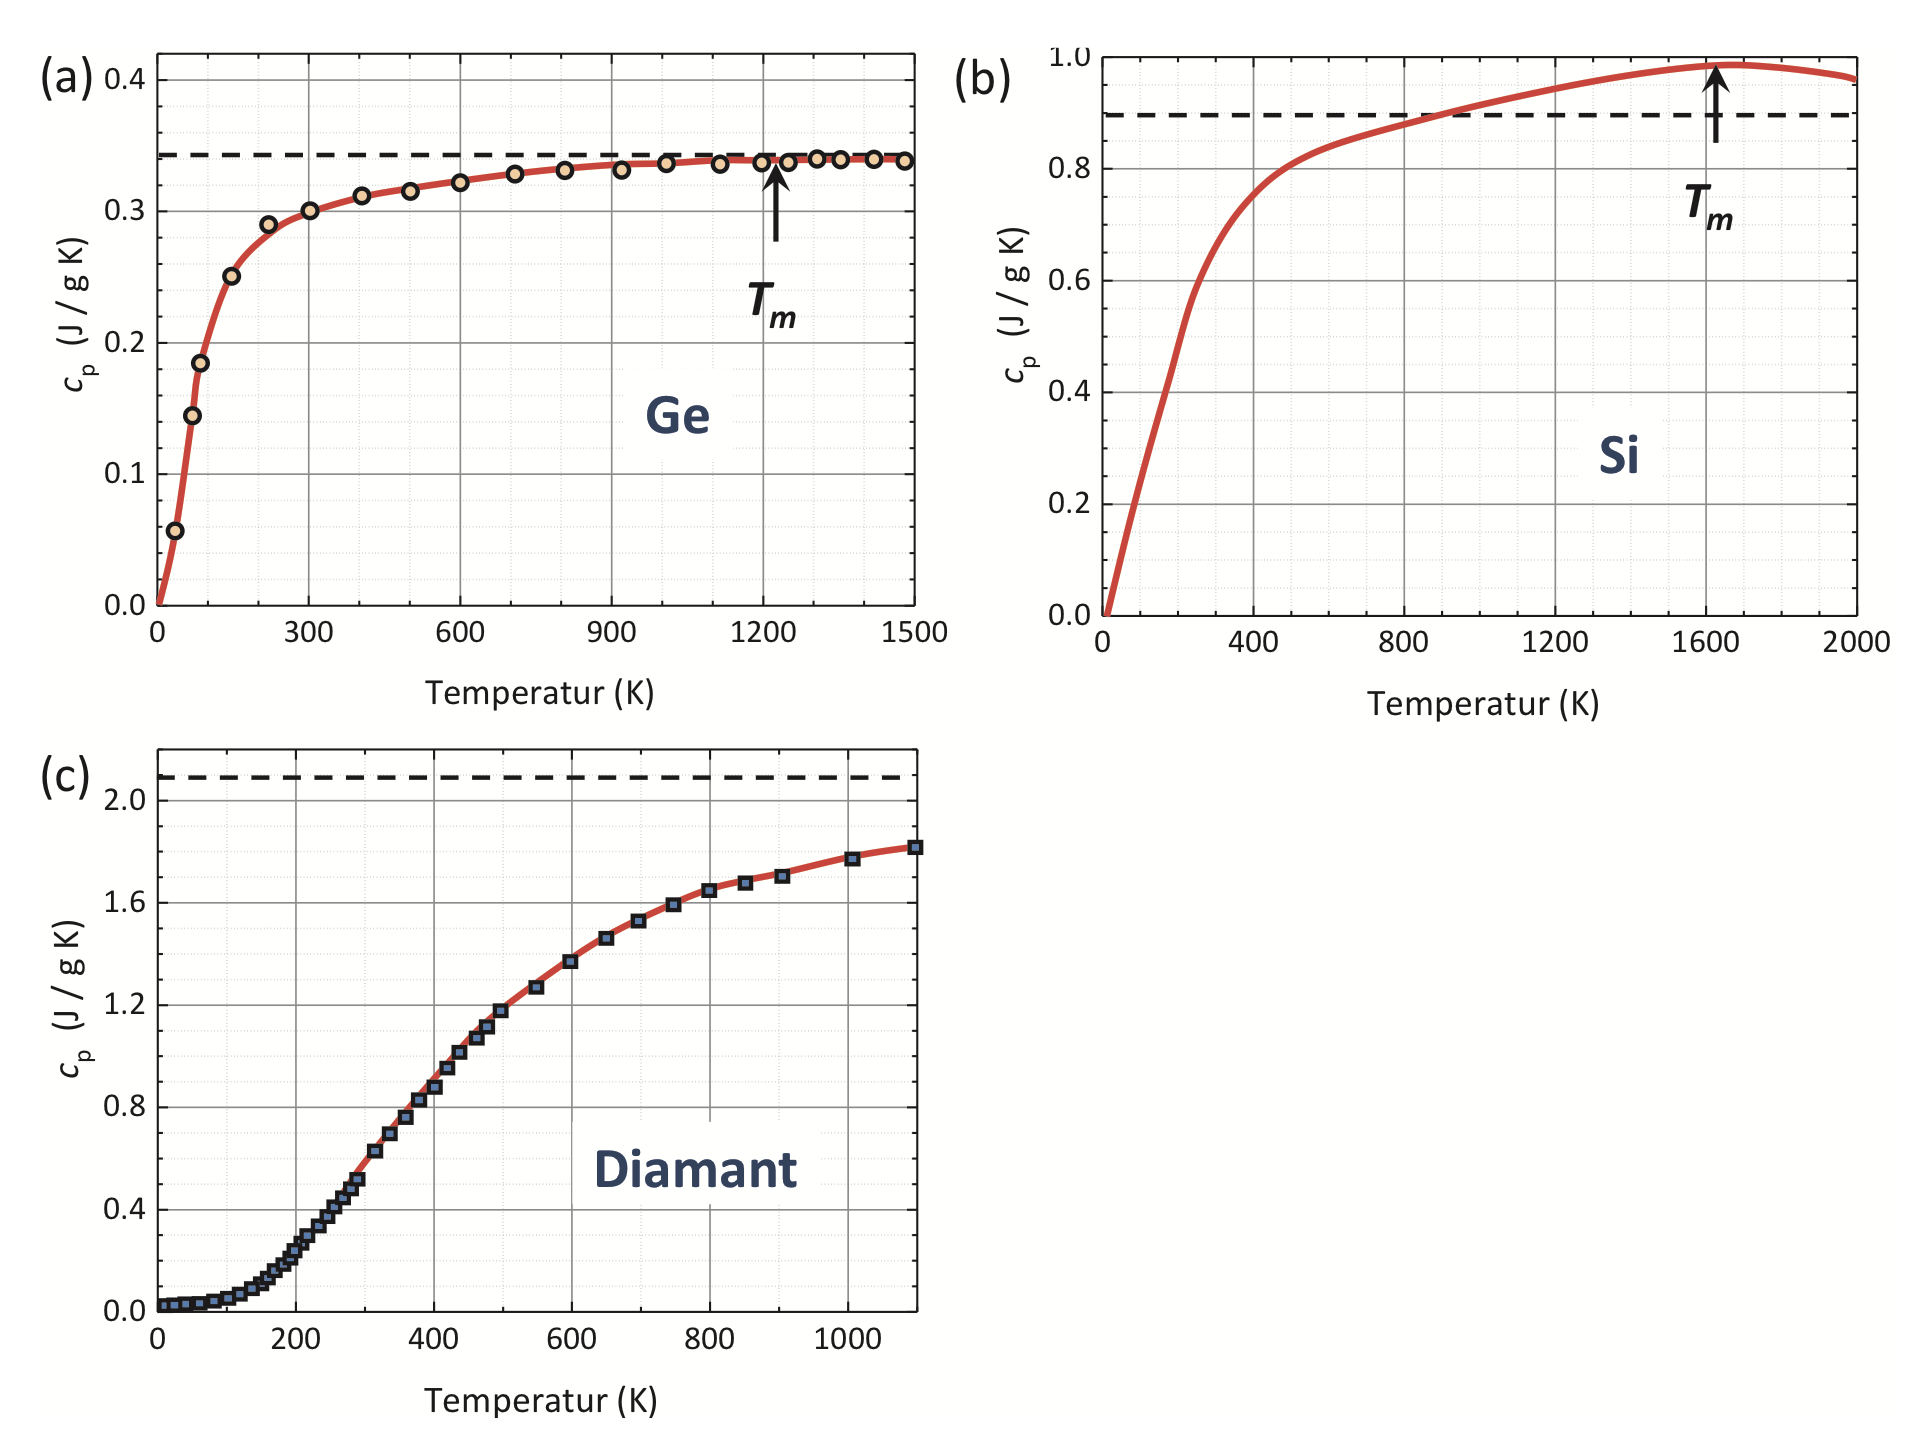
\includegraphics[scale=0.4]{content/V47_pictures/heat_capacity.png}
    \caption{In this figure we can see the temperature-dependece of the specific heat capacity $C_\mathrm{p}$ for different solids. \cite{grossmarx}}
    \label{fig:heat_cap_measurement}
\end{figure}

From the measurement, we can see that the classical limit, which means for high temperatures, the Dulong-Petit law is valid. Small deviations come due to anharmonic effects dominating
for higher $T$. But the significant perception is, that for low temperatures $C_\mathrm{V} \propto T^3$. Therefore \enquote{new physics} must be the explaination. With the idea of qunantization
of classically continuous phenomena a new idea for the calculation of the inner energy in a solid state system came up.

\section{Quantummechanical Theory of the Heat Capacity}
\label{sec:quantum}
Now we want to look at the quantized nature of lattice vibrations, so called \textit{Phonons}. Even so the Dulong-Petit model cannot describe the heat capacity for low temperatures,
the approach over the energy of lattice vibrations is not incorrect. We can describe the vibrations not as classcial oscillators, but as quantummechanical oscillators. Therefore the 
states in the low temperature regime are quantized, because $\hbar\omega >> k_\mathrm{B}T$. With this idea we can describe the solid state as an system of $3N$ harmonic oscillators.
To calculate the inner energy of such a system we can use Bose-Einstein-statistics. The inner energy in the low temperature regime is fundamentally dependent on the phonon dispersion.
In a solid state system there are always $3N - 3$ optical modes and $3$ acoustic modes. The common dispersion relation of phonons is shown in \autoref{fig:phonondispersion}. The general
approach to calculate the inner energy of this system would be using $D(E)\mathrm{d}E = Z(\vec{k})\mathrm{d^3}\vec{k}$ and integrating over the energy to get the inner energy. But 
calculating this without approximations is not possible.

\begin{figure}
    \centering
    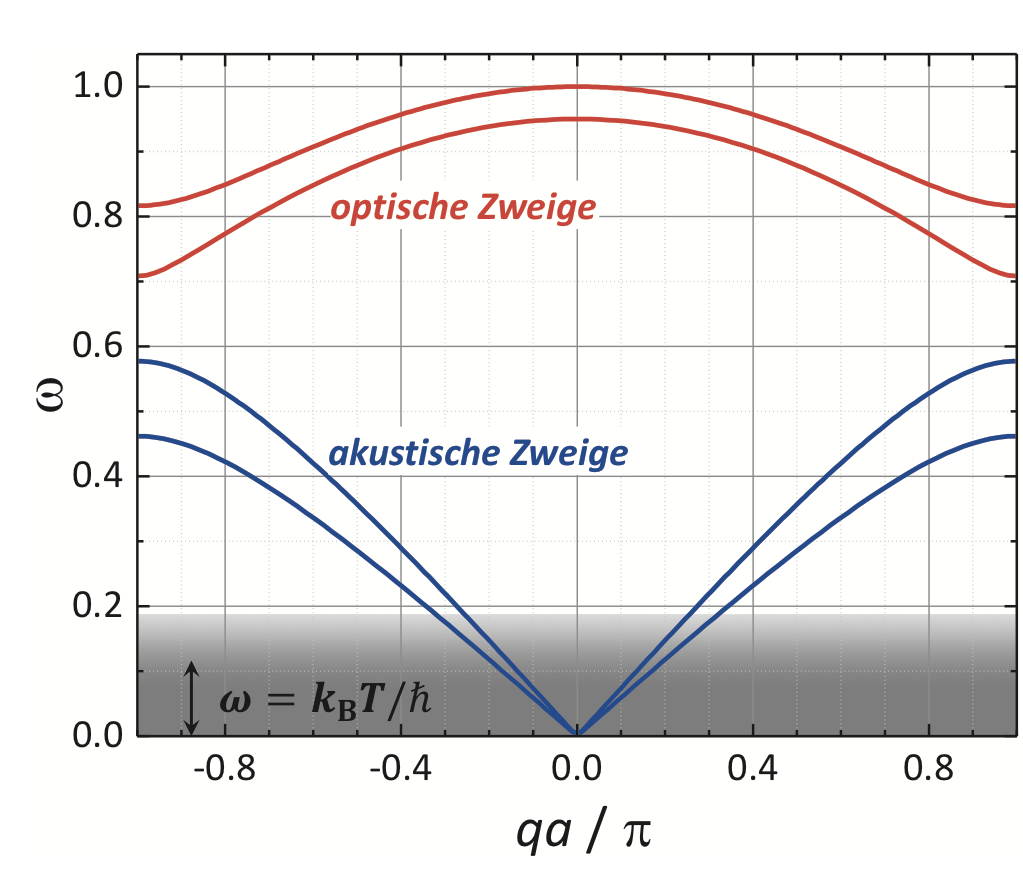
\includegraphics[scale=0.4]{content/V47_pictures/phonondispersion.png}
    \caption{In this figure we can see the phonon dispersionrelation for acoustic and optical modes. \cite{grossmarx}}
    \label{fig:phonondispersion}
\end{figure}

There are two common approximations to calculate the inner energy of a solid. The \enquote{Einstein-Approximation} and the \enquote{Debye-Approximation}.

\section{Einstein Approximation}
\label{sec:einstein}
The Einstein Approximation is based in the simple idea, that all the $3N$ phonon modes of the lattice have the same constant frequency $\omega_\mathrm{E}$. This means, that we have
state density given by equation \ref{eqn:den_einstein}.
\begin{equation}
    \label{eqn:den_einstein}
    D(\omega) = 3N\delta(\omega - \omega_\mathrm{E})
\end{equation}
With this state density we can calculate the inner energy with the before mentioned approach, which yields 
$\langle E \rangle = 3N\hbar\omega_\mathrm{E}(\frac{1}{2}+\frac{1}{e^{\hbar\omega_\mathrm{E}/k_\mathrm{B}T}-1})$. From this we can calculate the specific heat capacity with equation 
\ref{eqn:state_func}. To make so solution easier we define the \enquote{Einstein-temperature} $\Theta_\mathrm{E} = \frac{\hbar\omega}{K_\mathrm{B}}$. The specific heat capacity 
calculated using the Einstein-Approach results in equation \ref{eqn:einstein_heatcap}.
\begin{equation}
    \label{eqn:einstein_heatcap}
    C_{\mathrm{V}}^{\mathrm{E}} = 3Nk_\mathrm{B}\left(\frac{\Theta_\mathrm{E}}{T}\right)^2\frac{e^{\frac{\Theta_\mathrm{E}}{T}}}{\left(e^{\frac{\Theta_\mathrm{E}}{T}}-1\right)^2}
\end{equation} 

From equation \ref{eqn:einstein_heatcap} we can discuss the high and low temperature limits. These are given by the following equation.

\begin{equation*}
    C_{\mathrm{V}}^{\mathrm{E}} =
    \begin{cases}
        3Nk_\mathrm{B}\left(\frac{\Theta_\mathrm{E}}{T}\right)^2 e^{\frac{\Theta_\mathrm{E}}{T}} & \text{for } T <<  \Theta_\mathrm{E} \\
        3Nk_\mathrm{B} & \text{for } T >>  \Theta_\mathrm{E}
    \end{cases}
\end{equation*}

In the first case we see, that in this approximation we get an strong drop of the heat capacity for low temperatures. From measurements we know, that the heat capacity follows an $T^3$ proportionality,
which is not the result. But in generel this is an better description of the nature than Dulong-Petit. As for the other case, which is the \textit{calssical limit}, we optain the 
Law of Dulong-Petit. This shows, that even with this strong approximation we still get a better result than the classical approach.

\section{Debye-Approximation}
\label{sec:debye}
The Debye-Approximation has the idea to look at the low temperature limit, because this is where the classcial theory deviates from the measurement. In the low temperature regime the 
occupation of optical phonon modes is low. Due to that it is a good approximation to just use the $3$ acoustic phonon modes. The dispersion of acoustic phonons is proportional to  
$\lvert\text{sin}x\rvert$. For small temperatures the argument of the sinus is very small. Due to the small angle approximation it is valid to assume a linear dispersion for acoustic
phonons. Also the sum over all wavevectors can go over to an integral og the first Brillouin-Zone. This is the Debye Approximation. Due to the finiteness of a solid we can define
a cutoff frequency $w_{mathrm{D}}$ which is given by equation \ref{eqn:cutoff_freq}.
\begin{equation}
    \label{eqn:cutoff_freq}
    \int_0^{w_{\mathrm{D}}}D(\omega)\mathrm{d}\omega = 3N_\mathrm{L}
\end{equation}

In this equation $N_\mathrm{L}$ is the Loschmidt-constant. We can calculate the state density $D(\omega)$ using the approach with the linear dispersion. We know, that the state 
density in frequency domain is given by equation \ref{eqn:freq_dens}.
\begin{equation}
    \label{eqn:freq_dens}
    Z(\omega)\mathrm{d}\omega = \frac{V}{2\pi^2}\omega^2\left(\frac{1}{v_{\text{long}}^3}+\frac{2}{v_{\text{long}}^3}\right)
\end{equation} 

Since we only look at the longitudinal(acoustic) modes we can rewrite equation \ref{eqn:freq_dens} using the Debye frequency $\omega_\mathrm{D}$. This formula is shown in equation \ref{eqn:Z_w}.
\begin{equation}
    \label{eqn:Z_w}
    Z(\omega)\mathrm{d}\omega = \frac{9N_\mathrm{L}}{\omega_{\mathrm{D}}^3}\omega^2\mathrm{d}\omega
\end{equation}
With this state density we can calculate the energy of the solid and by deriving that for the temperature we can optain the heat capacity in the Debye-model. It is shown in equation 
\ref{eqn:heatcap_debye}.
\begin{equation}
    \label{eqn:heatcap_debye}
    C_{\mathrm{V}}^{\mathrm{D}} = \frac{\partial}{\partial T}\frac{9N_\mathrm{L}}{\omega_{\mathrm{D}}^3} \int_0^{\omega_{\mathrm{D}}}\frac{\omega^3}{e^{\hbar\omega/k_\mathrm{B}T}-1}
\end{equation}

From this equation we can discuss the two limits. The formula for each limit is shown in equation \ref{eqn:deb_limits}. We see, that the debye approximation results in an $\propto T^3$, 
which describes the natrue very good. Also the classical limit is the Dulong-Petits law.
\begin{equation}
    \label{eqn:deb_limits}
    C_{\mathrm{V}}^{\mathrm{D}} =
    \begin{cases}
        \frac{12\pi^4}{5}Nk_\mathrm{B}\left(\frac{T}{\Theta_\mathrm{D}}\right)^3 & \text{for } T <<  \Theta_\mathrm{D} \\
        3Nk_\mathrm{B} & \text{for } T >>  \Theta_\mathrm{D}
    \end{cases}
\end{equation}

The upper equation is defined in units of $\frac{T}{\Theta_\mathrm{D}}$. It is in units of the debye-temperatur, which is defined in equation \ref{eqn:theta_d}.
\begin{equation}
    \label{eqn:theta_d}
    \Theta_\mathrm{D} = \frac{\hbar\omega_\mathrm{D}}{k\mathrm{B}}
\end{equation} 
 It is a material specific value, characterizing its thermodynamic quantities.
\section{Comparrison of the Debye and Einstein Model}
\label{sec:comp_DE}
Both the Einstein and Debye-model use simple approximations to calculate the specific heat capacity. As seen in \autoref{fig:comp} the Debye model describes the nature better than Einstein, 
but for the extent of the approximations Einstein made both models have their own advantage for the low temperature regime. For high temperatures both models are equal. \autoref{fig:comp}
also shows the heat capacity for an free electron gas. A metal, such as copper, can be described using the free electron gas. Therefore we can see, that effects of the electron gas 
only plya a role in the very low temperature regime.
\begin{figure}
    \centering
    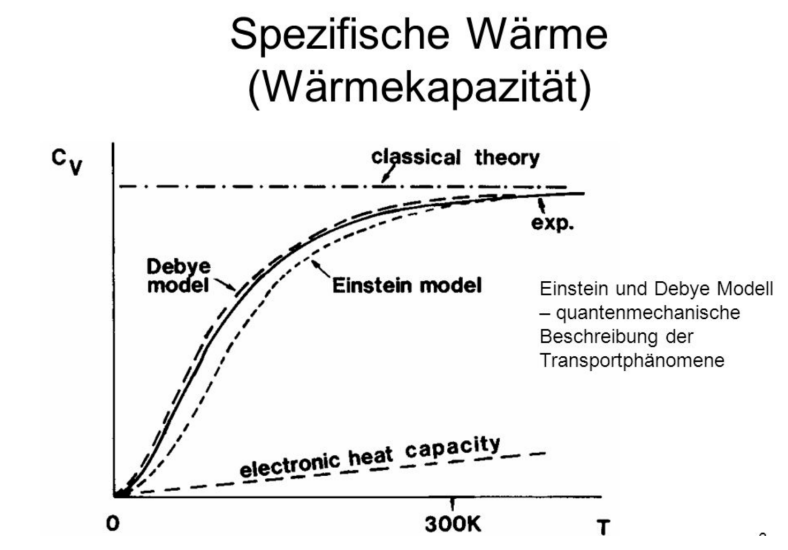
\includegraphics[scale=0.4]{content/V47_pictures/comp.PNG}
    \caption{In this figure we can see the function of the heat capacity for classical calculation and in the Einstein/Debye model.}
    \label{fig:comp}
\end{figure}